\section{Visão Geral}
\label{sec:estrategia_geral}

Para a implementação do interpretador, as tarefas necessárias para a
interpretagção, do código fonte ao resultado final de uma computação, foram
divididas entre quatro módulos: o Leitor, o Compilador, a Máquina Virtual e o
Sistema de Gerência de Memória.


O Leitor é responsável pela primeira etapa antes da compilação propriamente
dita: traduzir o código em formato textual fornecido pelo usuário para
Expressões-S. Durante a fase de leitura é realizada a análise léxica, bem como
a formação das listas que compõe a estrutura de um programa Scheme, que
corresponde a parte da análise sintática. O módulo Leitor é descrito em mais
detalhes na seção \ref{sec:leitor}.

Utilizando as Expressões-S geradas pelo Leitor, identifica qual estrutura da
linguagem cada Expressão-S representa, reconhece instâncias de macros que devem
ser traduzidas para as definições dadas pelo usuário e finalmente gera o código
que deve ser executado para avaliação das expressões fornecidas. Como a
tradução de macros acontece antes da geração de código, esta fase fica
significativamente mais simples, precisando apenas lidar com as poucas
estruturas primitivas que a linguagem define, deixando as demais para serem
reduzidas às estruturas primitivas por meio de macros. Na seção
\ref{sec:compilador} são fornecidos mais detalhes sobre o Compilador, bem como
seus sub-módulos: o Leitor e o Sistema de Macros.

A Máquina Virtual, então, é encarregada de avaliar as operações codificadas em
instruções básicas, utilizando o código gerado pelo compilador, e retornar o
valor desta avaliação. Para tanto, esta depende de um contexto de execução,
composto das ligações presentes no escopo global. Informações extras de
contexto, como os escopos locais e estado da pilha de controle, entre outras,
são mantidas e serão discutidas, junto com uma descrição detalhada da Máquina
Virtual, na seção \ref{sec:maquina-virtual}.

Uma representação simplificada do funcionamento do interpretador, baseada na descrição acima, pode
ser vista na figura \ref{fig:visao-geral-implementacao}.

\begin{figure}[h!]
\centering
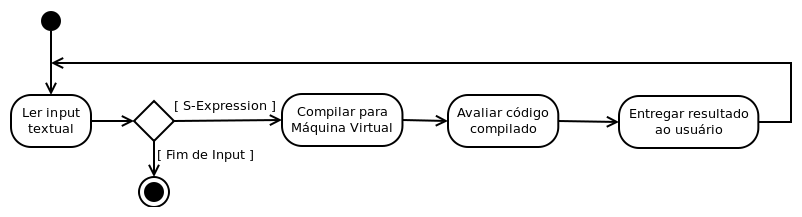
\includegraphics[width=0.9\textwidth]{../images/visao-geral-implementacao.pdf}
\caption{Visão geral do funcionamento interno do interpretador}
\label{fig:visao-geral-implementacao}
\end{figure}

Os módulos descritos acima são implementados sobre o sistema de Gerência de
Memória. A Gerência de Memória é baseada em uma implementação simples do
algoritmo de Mark \& Sweep [17], em que a memória livre é armazenada como uma
lista encadeada de nós de memória de tamanho único (neste caso, 24 bytes). Com
a ajuda de um conhecimento mais íntimo da máquina virtual em questão, o sistema
de gerência de memória pode então, quando necessário, identificar quais nós de
memória estão em uso e liberar para uso posterior todos os demais. Na seção
\ref{sec:memoria} detalharemos o sistema de memória, embora uma compreensão
completa do mesmo só seja possível após indicarmos quais partes da máquina
virtual estão envolvidas no processo de identificar quais nós de memória estão
em uso.

Podemos ter então, quebrando o trabalho do compilador em seus sub módulos
separadamente, uma visão geral da arquitetura do Interpretador, em como os
módulos se relacionam na figura \ref{fig:camadas} e de como se dá, em detalhes, o
processo de interpretação de uma expressão Scheme dada como entrada ao
interpretador na figura \ref{fig:atividades}

\begin{figure}[h!]
\centering
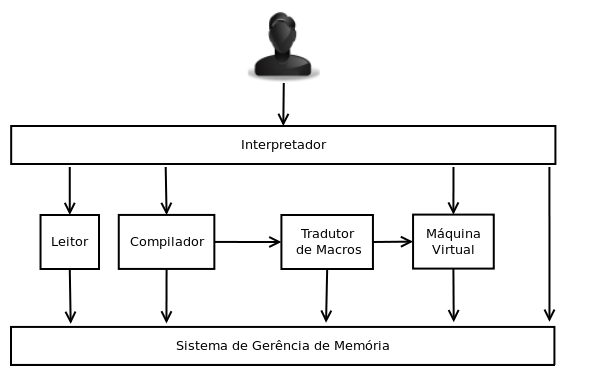
\includegraphics[width=0.9\textwidth]{../images/camadas.pdf}
\caption{Estrutura e relacionamento entre os módulos do interpretador}
\label{fig:camadas}
\end{figure}

\begin{figure}[h!]
\centering
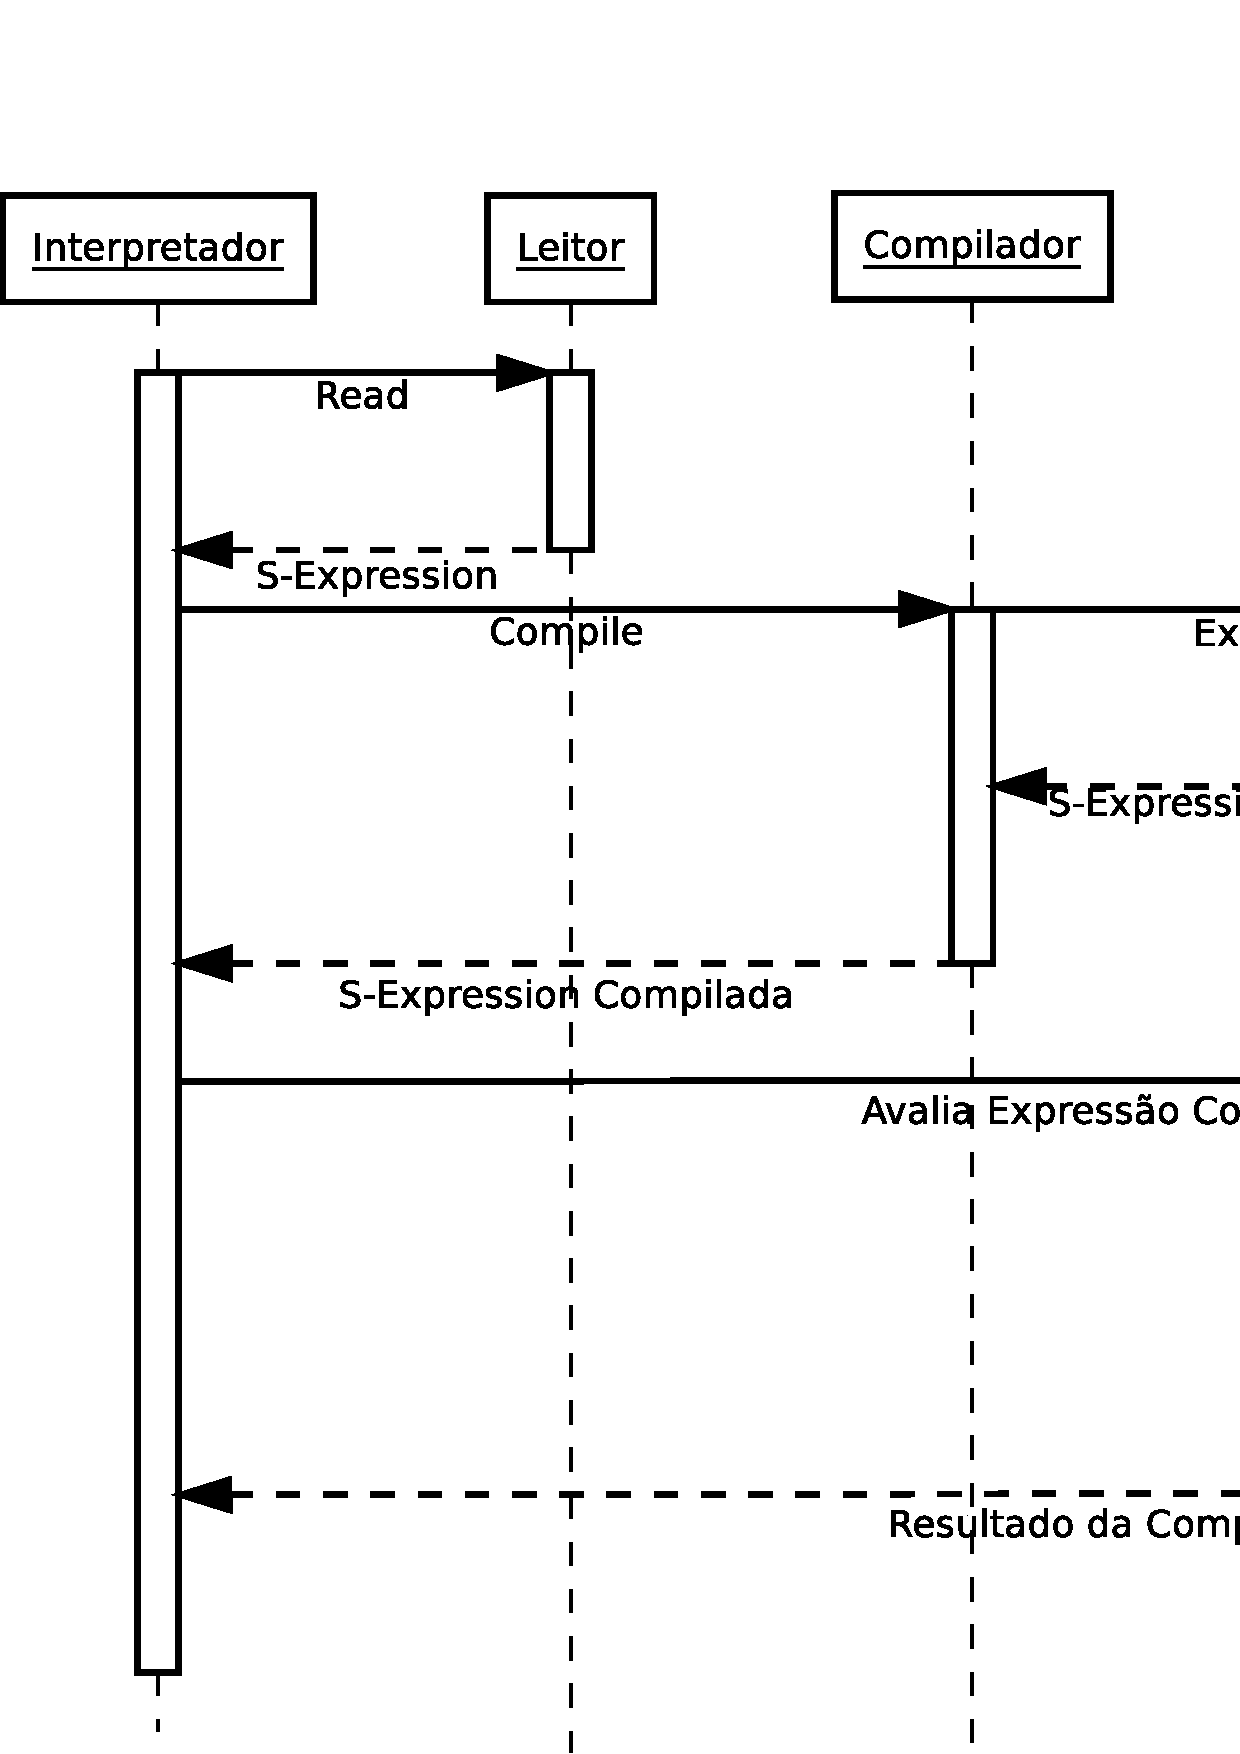
\includegraphics[width=0.9\textwidth]{../images/atividades.pdf}
\caption{Processo interno de interpretação}
\label{fig:atividades}
\end{figure}

A implementação do interpretador baseado no esquema descrito acima se dá em um
ambiente de duas linguagens: C++ e Scheme.

A estrutura básica do interpretador, até o ponto em que este é capaz de
interpretar um pequeno conjunto de operações básicas, é feito em C++. Esta
estrutura inclui todo o mecanismo de gerência de memória, o leitor, o
compilador para as estruturas sintáticas primitivas e a máquina virtual, além
de um pequeno conjunto de funções primitivas que são mais fácilmente
implementadas em C++ por apenas delegarem o trabalho para funções e operadores
primmitivos desta linguagem.

A partir deste ponto, as demais estruturas sintáticas são escritas na forma de
macros em Scheme e diversas funções da biblioteca são implementadas em código
Scheme que roda no próprio interpretador. 

Utilizando uma análise de número de linhas de código, que não é exatamente
representativa dada a diferença de expressividade das duas linguagens,
aproximadamente 88\% da implementação é feita em C++, enquanto que os 12\%
restantes são feitos em Scheme.



